\section{Istruzioni all'uso}
% \subsection{Login}
\subsection{Home}
All'avvio dell'applicazione si è portati alla pagina "Home". Da qui si può accedere a vari strumenti, tra cui la barra di ricerca, la barra degli strumenti, le varie dashboard disponibili e al menù a tendina presente in angolo a sinistra.
\begin{center}
    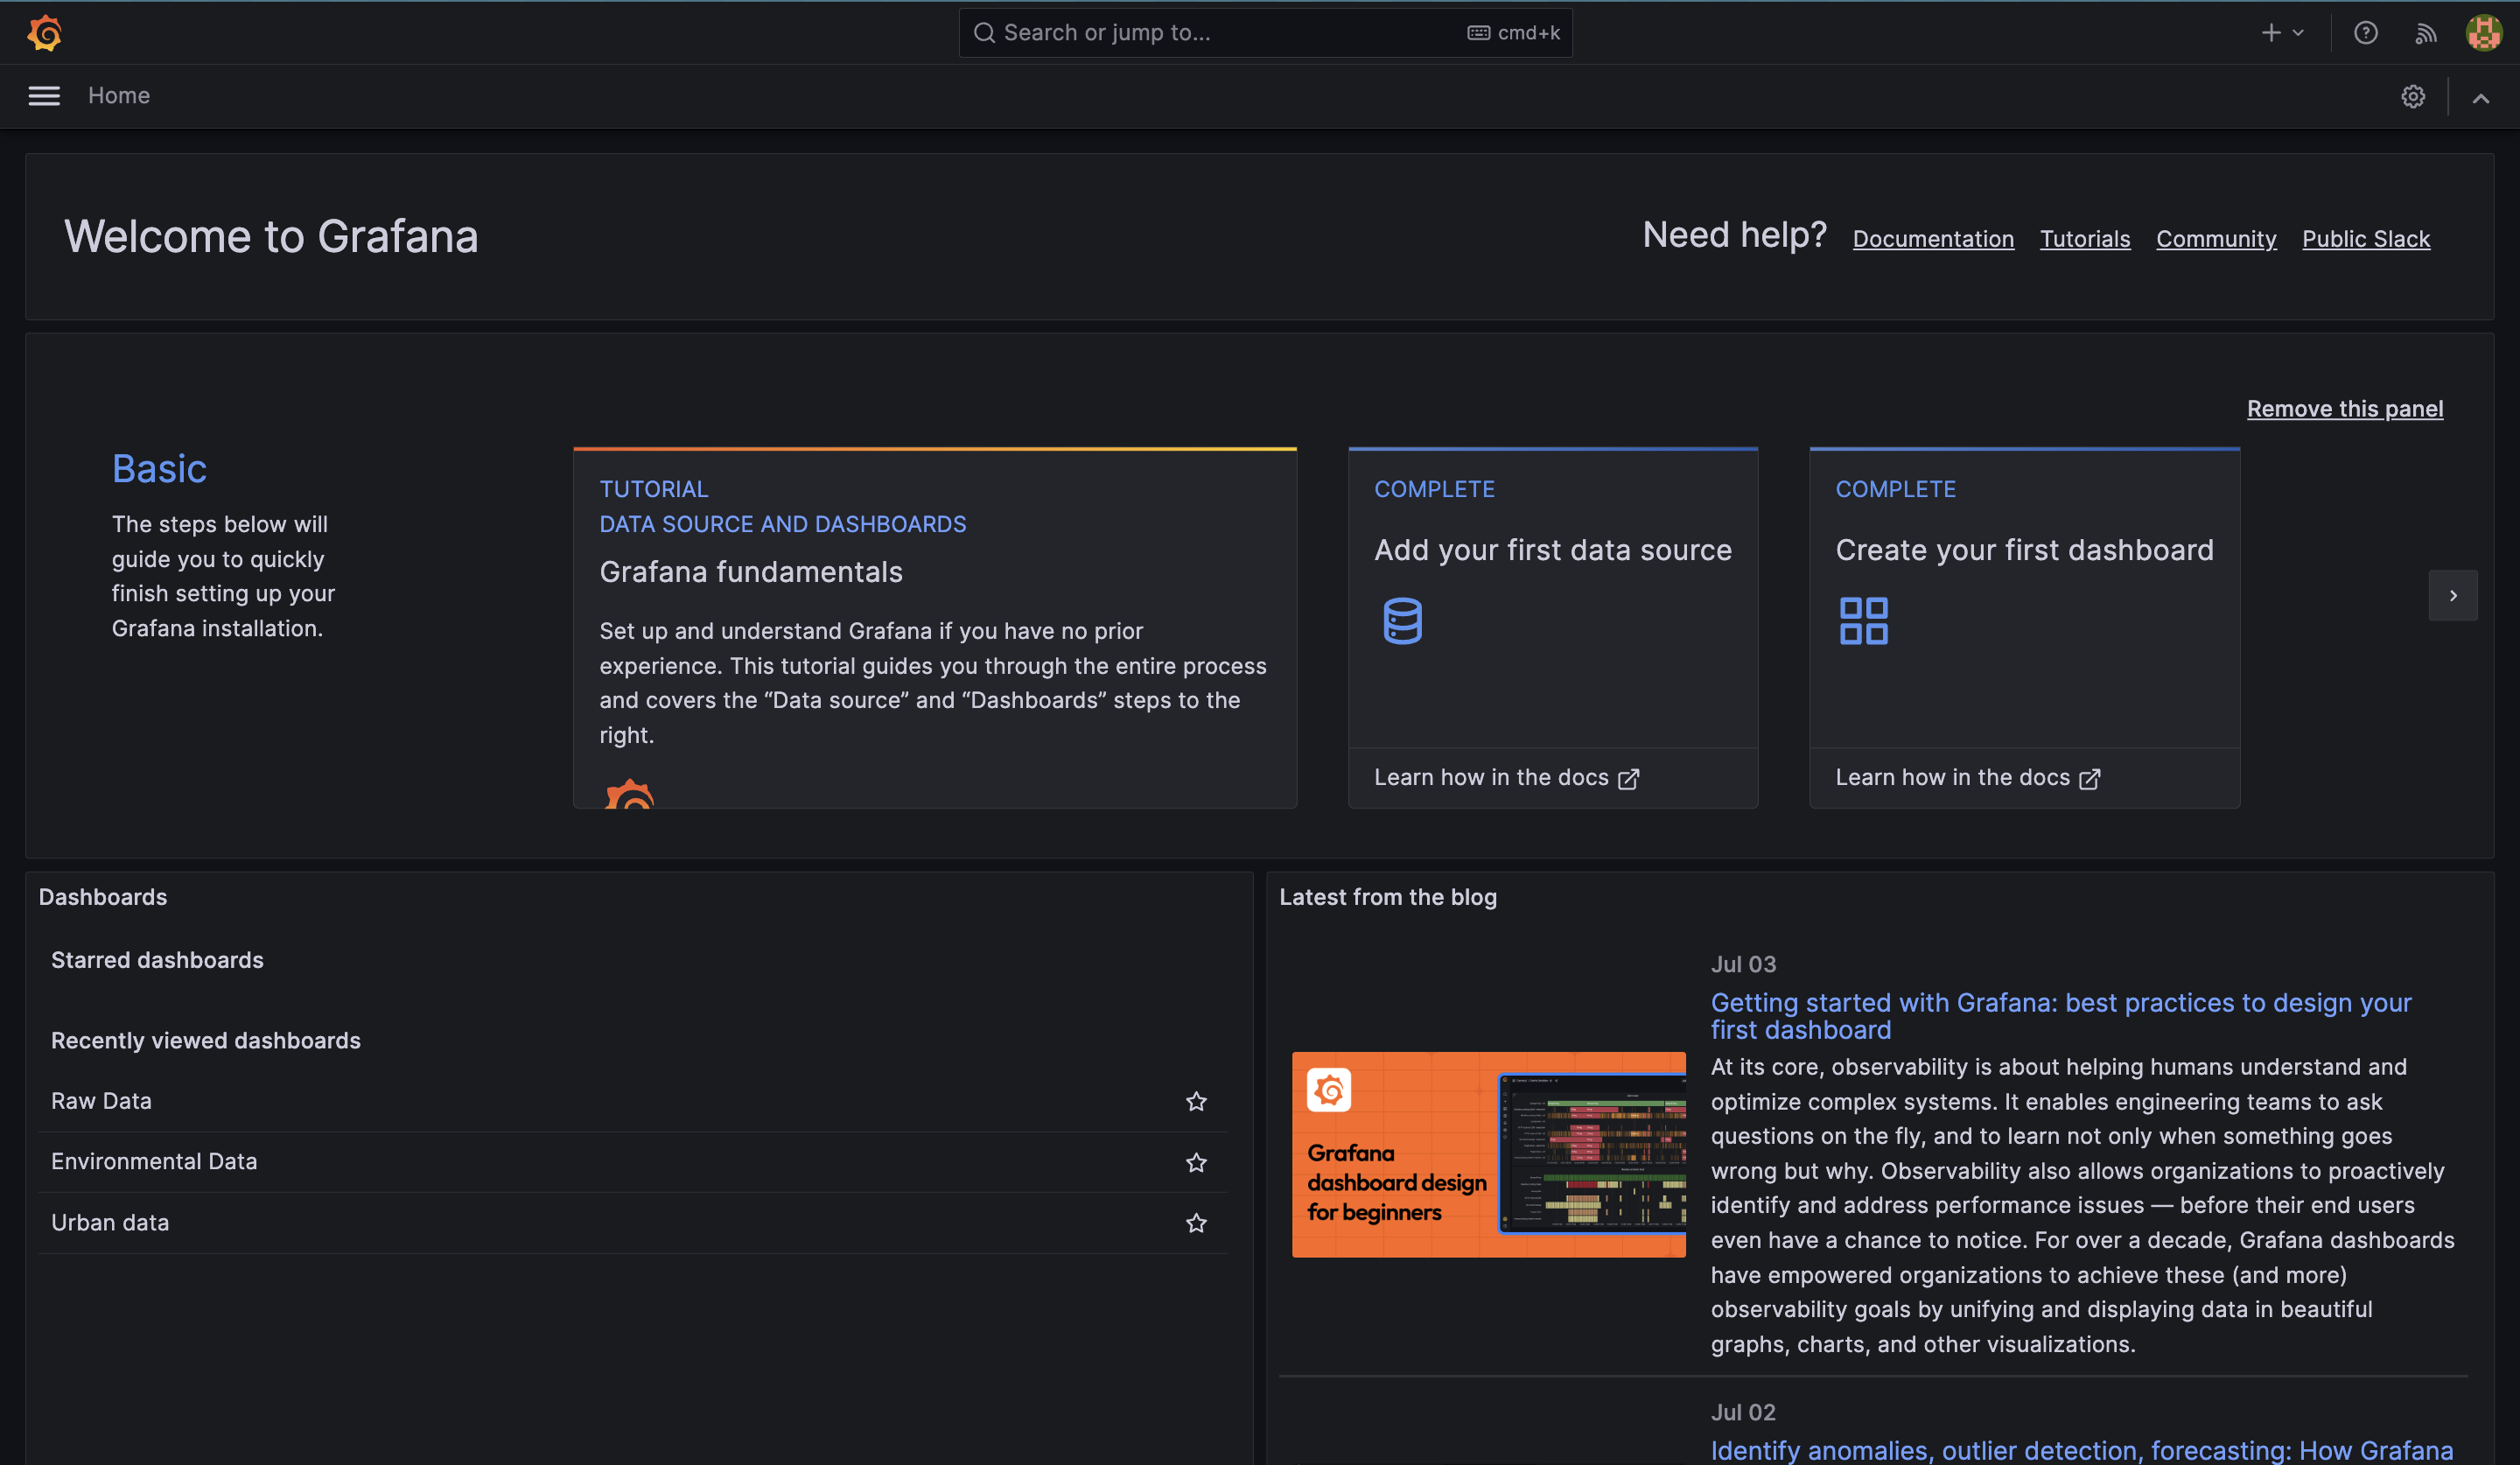
\includegraphics[width=\textwidth]{manuale/home.png}
    \captionof{figure}{Schermata di accesso}
\end{center}
\newpage
\subsubsection{Barra di ricerca}
Questo strumento permette un filtraggio rapido e preciso delle varie pagine presenti nell'applicazione. 
\begin{center}
    
\includegraphics[width=0.6\textwidth]{manuale/barra_ricerca.png}
    \captionof{figure}{Barra di ricerca}
\end{center}

\subsubsection{Barra degli strumenti}
La barra degli strumenti è progettata per fornire all'utente un accesso immediato a una serie di funzionalità e azioni utili. Qui si possono trovare opzioni per personalizzare la visualizzazione dei dati, eseguire interrogazioni avanzate, gestire allarmi e condividere i risultati.
\begin{center}
    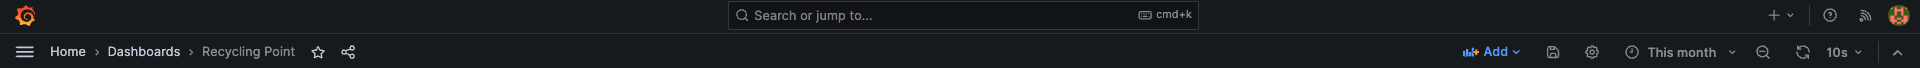
\includegraphics[width=\textwidth]{manuale/barra_strumenti.png}
    \captionof{figure}{Barra degli strumenti}
\end{center}
All'interno della barra degli strumenti si trovano ulteriori funzionalità, pensate per facilitare l'interazione con l'applicazione. Partendo da sinistra verso destra troviamo:
\begin{itemize}
    \item \textbf{Menù a tendina}, dove è possibile avere accesso ad alcune sezioni fondamentali per lo scopo ultimo di questo prodotto. Tra queste troviamo:
        \begin{itemize}
            \item \textbf{Starred}, contenente tutte le dashboard preferite;
            \item \textbf{Dashboards}, dove si trovano tutte le dashboard disponibili;
            \item \textbf{Alerting}, contenente tutte le notifiche e gli allarmi attivi.
        \end{itemize}
        \begin{center}
            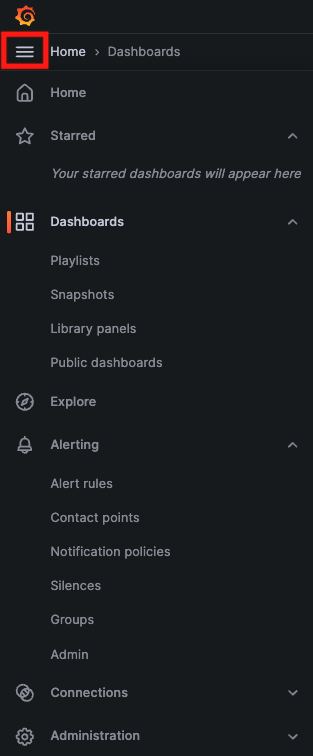
\includegraphics[width=0.2\textwidth]{manuale/menu_tendina.png}
            \captionof{figure}{Menù a tendina}
        \end{center}
    \item \textbf{Breadcrumb}, che mostra la posizione attuale dell'utente all'interno dell'applicazione.
        \begin{center}
            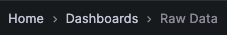
\includegraphics[width=0.6\textwidth]{manuale/breadcrumb.png}
            \captionof{figure}{Breadcrumb}
        \end{center}
    \item \textbf{Favorite mark}, che permette di aggiungere o rimuovere una dashboard dai preferiti.
        \begin{center}
            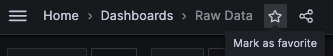
\includegraphics[width=0.6\textwidth]{manuale/favorite_mark.png}
            \captionof{figure}{Favorite mark}
        \end{center}
    \item \textbf{Share dashboard}, che consente di condividere la dashboard corrente con altri utenti.
        \begin{center}
            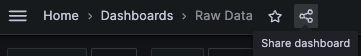
\includegraphics[width=0.6\textwidth]{manuale/share.png}
            \captionof{figure}{Share dashboard}
        \end{center}
    \item \textbf{Add button}, che permette di aggiungere un nuovo pannello alla dashboard corrente.
        \begin{center}
            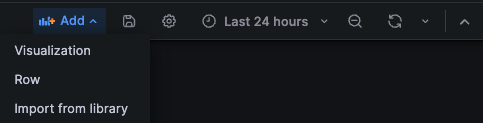
\includegraphics[width=0.6\textwidth]{manuale/add_button.png}
            \captionof{figure}{Add button}
        \end{center}
    \item \textbf{Save dashboard}, che consente di salvare le modifiche apportate alla dashboard corrente.
        \begin{center}
            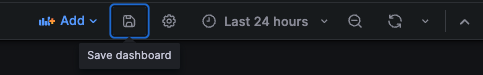
\includegraphics[width=0.6\textwidth]{manuale/save.png}
            \captionof{figure}{Salva dashboard}
        \end{center}
    \item \textbf{Impostazioni dashboard}, che permette di personalizzare la dashboard corrente.
        \begin{center}
            
\includegraphics[width=0.6\textwidth]{manuale/settings.png}
            \captionof{figure}{Impostazioni dashboard}
        \end{center}
    \newpage
    \item \textbf{Time range}, che consente di selezionare l'intervallo temporale dei dati visualizzati.
        \begin{center}
            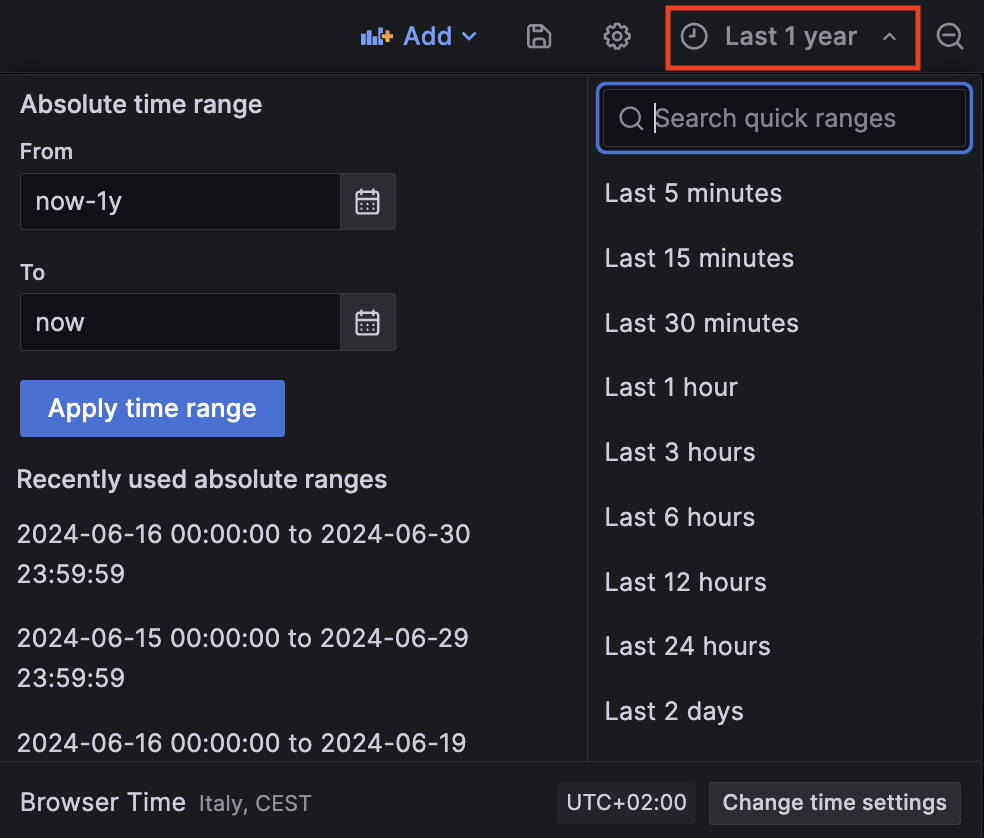
\includegraphics[width=0.6\textwidth]{manuale/time_range.png}
            \captionof{figure}{Time range}
        \end{center}
    \item \textbf{Refresh}, che permette di aggiornare i dati visualizzati.
        \begin{center}
            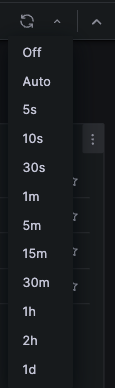
\includegraphics[width=0.1\textwidth]{manuale/refresh.png}
            \captionof{figure}{Refresh}
        \end{center}
\end{itemize}
% \subsubsection{Menù a tendina}
% All'interno di questo è possibile avere accesso ad alcune sezioni fondamentali per lo scopo ultimo di questo prodotto. Tra queste troviamo:
% \begin{itemize}
%     \item \textbf{Starred}, contenente tutte le dashboard preferite;
%     \item \textbf{Dashboards}, all'interno della quale si possono trovare tutte le dashboard disponibili;
%     \item \textbf{Alerting}, contenente tutte le notifiche e gli allarmi attivi;
% \end{itemize}
% \begin{center}
%     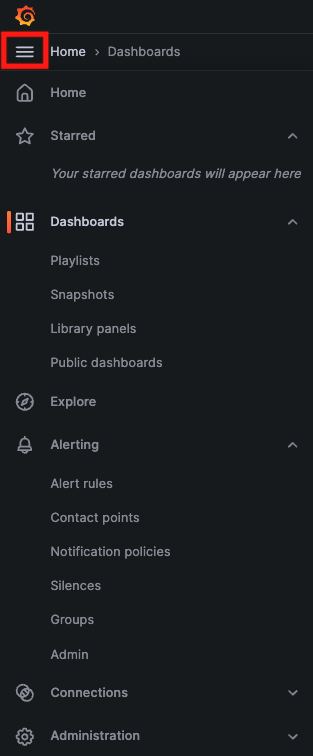
\includegraphics[width=0.3\textwidth]{manuale/menu_tendina.png}
%     \captionof{figure}{Menù a tendina}
% \end{center}
\newpage
\subsection{Dashboard}
Le dashboard sono la parte centrale dell'applicazione, progettate per fornire una visualizzazione intuitiva e dettagliata dei dati raccolti dai sensori. Ogni dashboard è composta da pannelli dedicati, ciascuno focalizzato su un aspetto specifico dell'analisi o del monitoraggio. Questi pannelli contengono grafici interattivi, tabelle e altre visualizzazioni che consentono agli utenti di esplorare i dati in modo efficace e approfondito.

\subsubsection{Pannelli}
All'interno di ogni dashboard sono presenti pannelli dedicati, ciascuno focalizzato su un insieme specifico di informazioni. Ogni pannello racchiude dati pertinenti rappresentati attraverso grafici o altre visualizzazioni, offrendo così una panoramica chiara e dettagliata su un determinato aspetto dell'analisi o del monitoraggio. Ciascun pannello contiene:
\begin{itemize}
    \item nome dello stesso;
    \item informazioni in merito al sensore;
    \item menù a tendina (se presente);
    \item legenda (se presente);
    \item visualizzazione dei dati misurati.
\end{itemize}

\subsubsection{Tipologie di grafici}
\subsubsubsection*{Mappa}
Questa visualizzazione rappresenta la posizione dei sensori su una mappa interattiva. Utilizzando i pulsanti "+" e "-" è possibile ingrandire e ridurre la mappa per visualizzare più dettagli o una vista più ampia, rispettivamente. Facendo clic su un marker del sensore, si apre un popup che fornisce informazioni dettagliate sul sensore corrispondente. È inoltre possibile spostarsi sulla mappa trascinando il mouse tenendo premuto, consentendo una navigazione fluida all'interno dell'area rappresentata. Nell'angolo in basso a sinistra è disponibile una legenda che identifica i diversi tipi di sensori presenti sulla mappa.
\begin{center}
    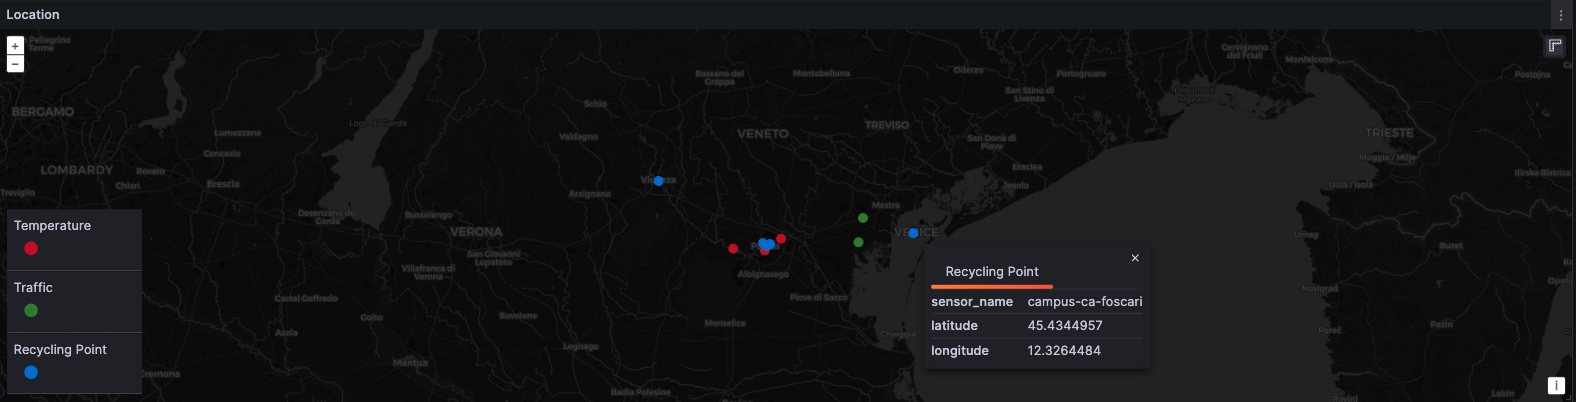
\includegraphics[width=\textwidth]{manuale/mappa.png}
    \captionof{figure}{Mappa dei sensori}
\end{center}

\subsubsubsection*{Grafico a linee} 
Questo tipo di visualizzazione rappresenta i dati in forma di linee, con l'asse x che rappresenta il tempo e l'asse y che rappresenta il valore misurato. È possibile visualizzare più serie di dati contemporaneamente, consentendo di confrontare facilmente i dati provenienti da diversi sensori o categorie.
\begin{center}
    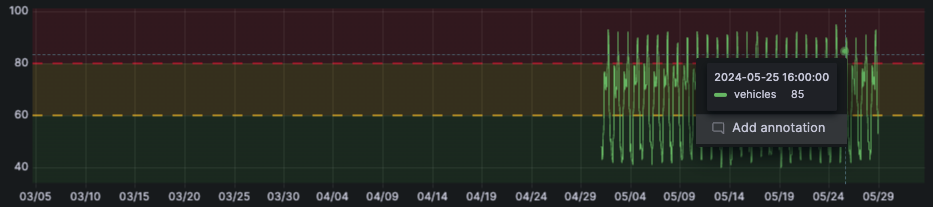
\includegraphics[width=\textwidth]{manuale/time_series.png}
    \captionof{figure}{Grafico a linee}
\end{center} 

\subsubsubsection*{Statistiche}
Fornisce un'istantanea del valore misurato, mostrando ad esempio un numero o un indicatore visivo come una freccia o un'icona. Utile per monitorare un singolo dato in tempo reale e per evidenziare eventuali anomalie o variazioni significative.
\begin{center}
    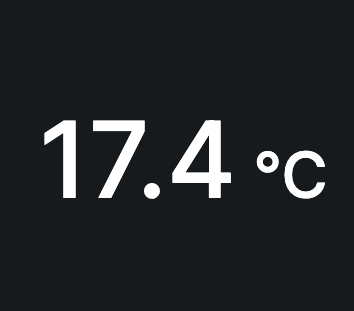
\includegraphics[width=0.4\textwidth]{manuale/stat.png}
    \captionof{figure}{Grafico per le statistiche}
\end{center} 

\subsubsubsection*{Grafico a quadrante}
Questo tipo di visualizzazione divide i dati in quattro quadranti, ciascuno rappresentato da un colore diverso. Ogni quadrante corrisponde a un intervallo di valori specifico, consentendo di identificare rapidamente se il valore misurato è inferiore, superiore o all'interno di un determinato intervallo. Particolarmente utile per valutare le prestazioni rispetto a obiettivi o soglie prestabilite.
\begin{center}
    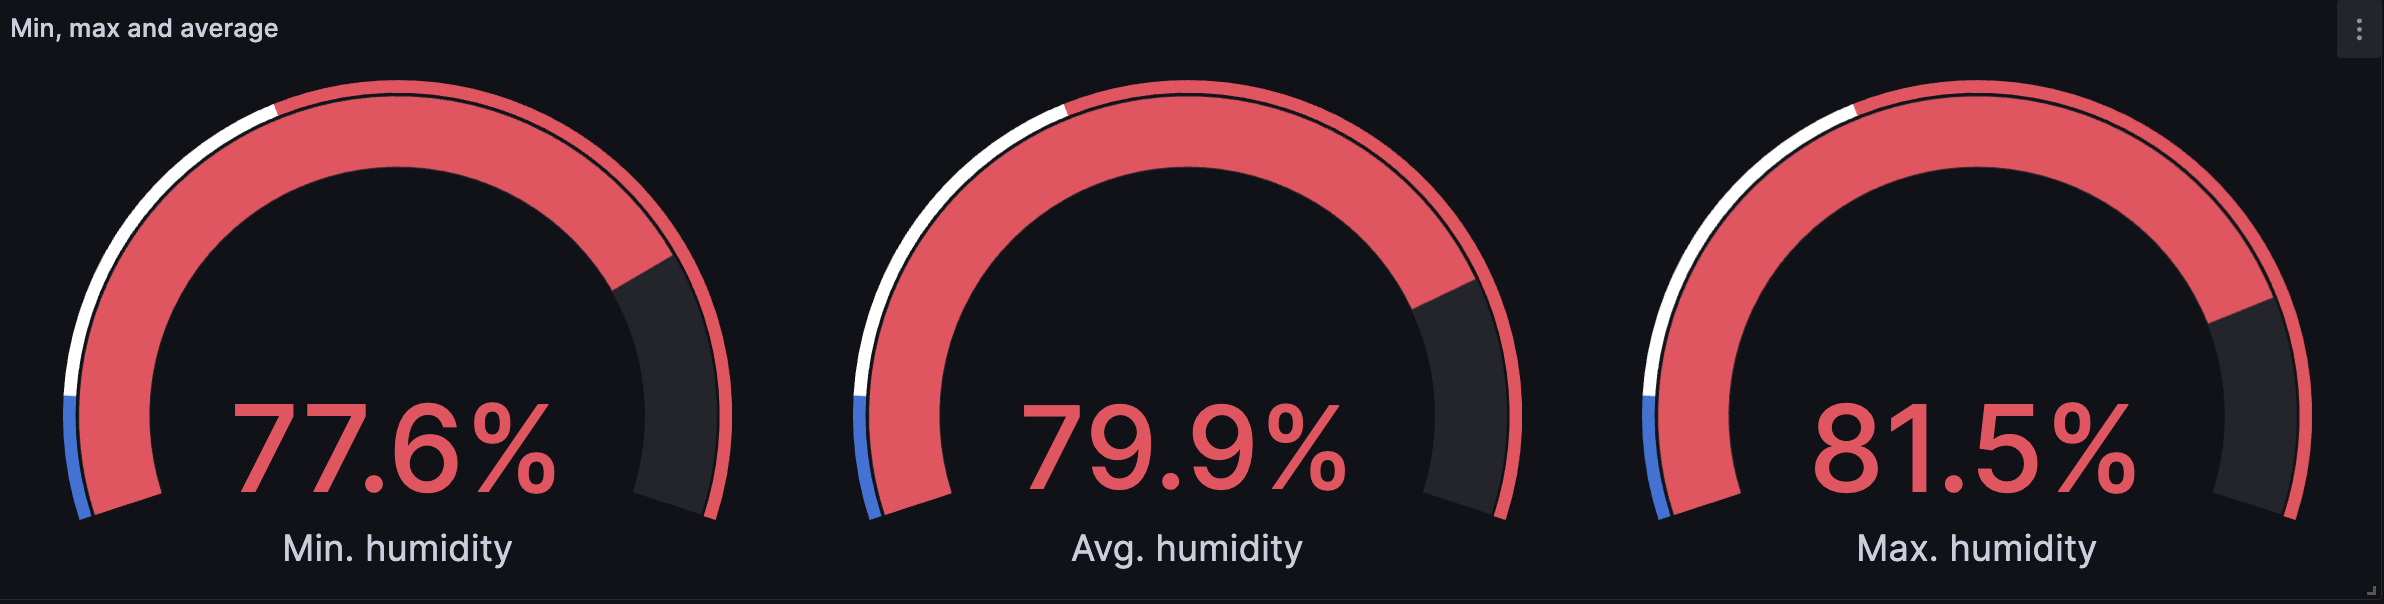
\includegraphics[width=\textwidth]{manuale/grafico_quadrante.png}
    \captionof{figure}{Grafico a quadrante}
\end{center}

\subsubsubsection*{Grafico a barre}
Questo tipo di visualizzazione rappresenta i dati in forma di barre orizzontali o verticali, con l'altezza o la lunghezza della barra proporzionale al valore misurato. 
\begin{center}
    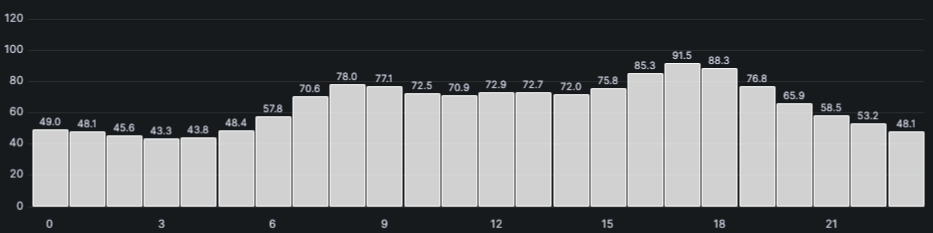
\includegraphics[width=\textwidth]{manuale/grafico_barre.png}
    \captionof{figure}{Grafico a barre}
\end{center}

\subsubsubsection*{Tabella}
Questa visualizzazione rappresenta i dati provenienti dai sensori in forma tabellare. Ogni riga della tabella corrisponde a un sensore e mostra le relative informazioni. Le colonne della tabella rappresentano le diverse categorie di dati, come valori misurati e timestamp della misurazione. La tabella fornisce una visione compatta e organizzata dei dati dei sensori, facilitando la ricerca e l'analisi delle informazioni.
\begin{center}
    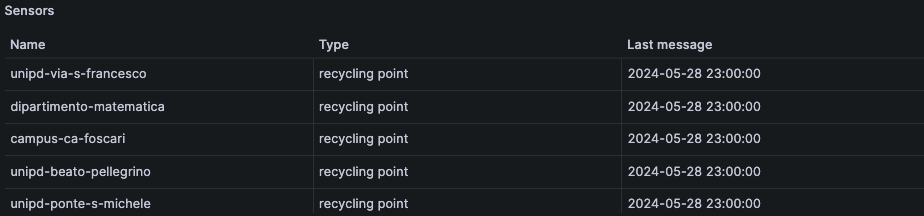
\includegraphics[width=\textwidth]{manuale/tabelle.png}
    \captionof{figure}{Tabelle}
\end{center} 


\subsubsection{Gestione sensori visualizzabili}
È stato progettato un filtro per consentire all'utente di visualizzare solo i sensori di interesse. Questo filtro è disponibile in ogni dashboard e consente di selezionare i sensori da visualizzare in base a diversi criteri, come il tipo di sensore, la posizione geografica o lo stato operativo. Questo filtro è particolarmente utile quando si lavora con un gran numero di sensori e si desidera concentrarsi solo su quelli rilevanti per l'analisi o il monitoraggio in corso.


\subsection{Gruppi di pannelli}
\subsubsection{Raw Data}
La dashboard generale consente di visualizzare la posizione dei sensori su una mappa interattiva, con codifica a colori per diverse tipologie di sensori, come temperatura, traffico e punti di riciclo. Include grafici dinamici per l'andamento temporale dei dati, tabelle dettagliate con informazioni aggiornate e statistiche riassuntive per una comprensione immediata. La sezione \textit{Raw Data} dall'alto verso il basso e da sinistra verso destra è composta da:
\begin{itemize}
    \item filtro per visualizzare i sensori di preferenza;
    \item mappa dei sensori;
    \item collegamento alle dashboard dettagliate;
    \item tabella con tutti i sensori e l'ultima rilevazione effettuata;
    \item grafico a barre orizzontali con il totale di sensori per tipo;
    \item tabella della temperatura con i valori misurati e la data della loro misurazione;
    \item grafico a linee con l'andamento della temperatura nel tempo;
    \item tabella per i sensori del traffico con i valori misurati e la data della loro misurazione;
    \item grafico a linee con l'andamento del traffico nel tempo;
    \item grafico a linee con la velocità del traffico nel tempo;
    \item tabella per i sensori delle isole ecologiche con i valori misurati e la data della loro misurazione;
    \item grafico a linee con l'andamento delle isole ecologiche nel tempo.
\end{itemize}
\begin{center}
    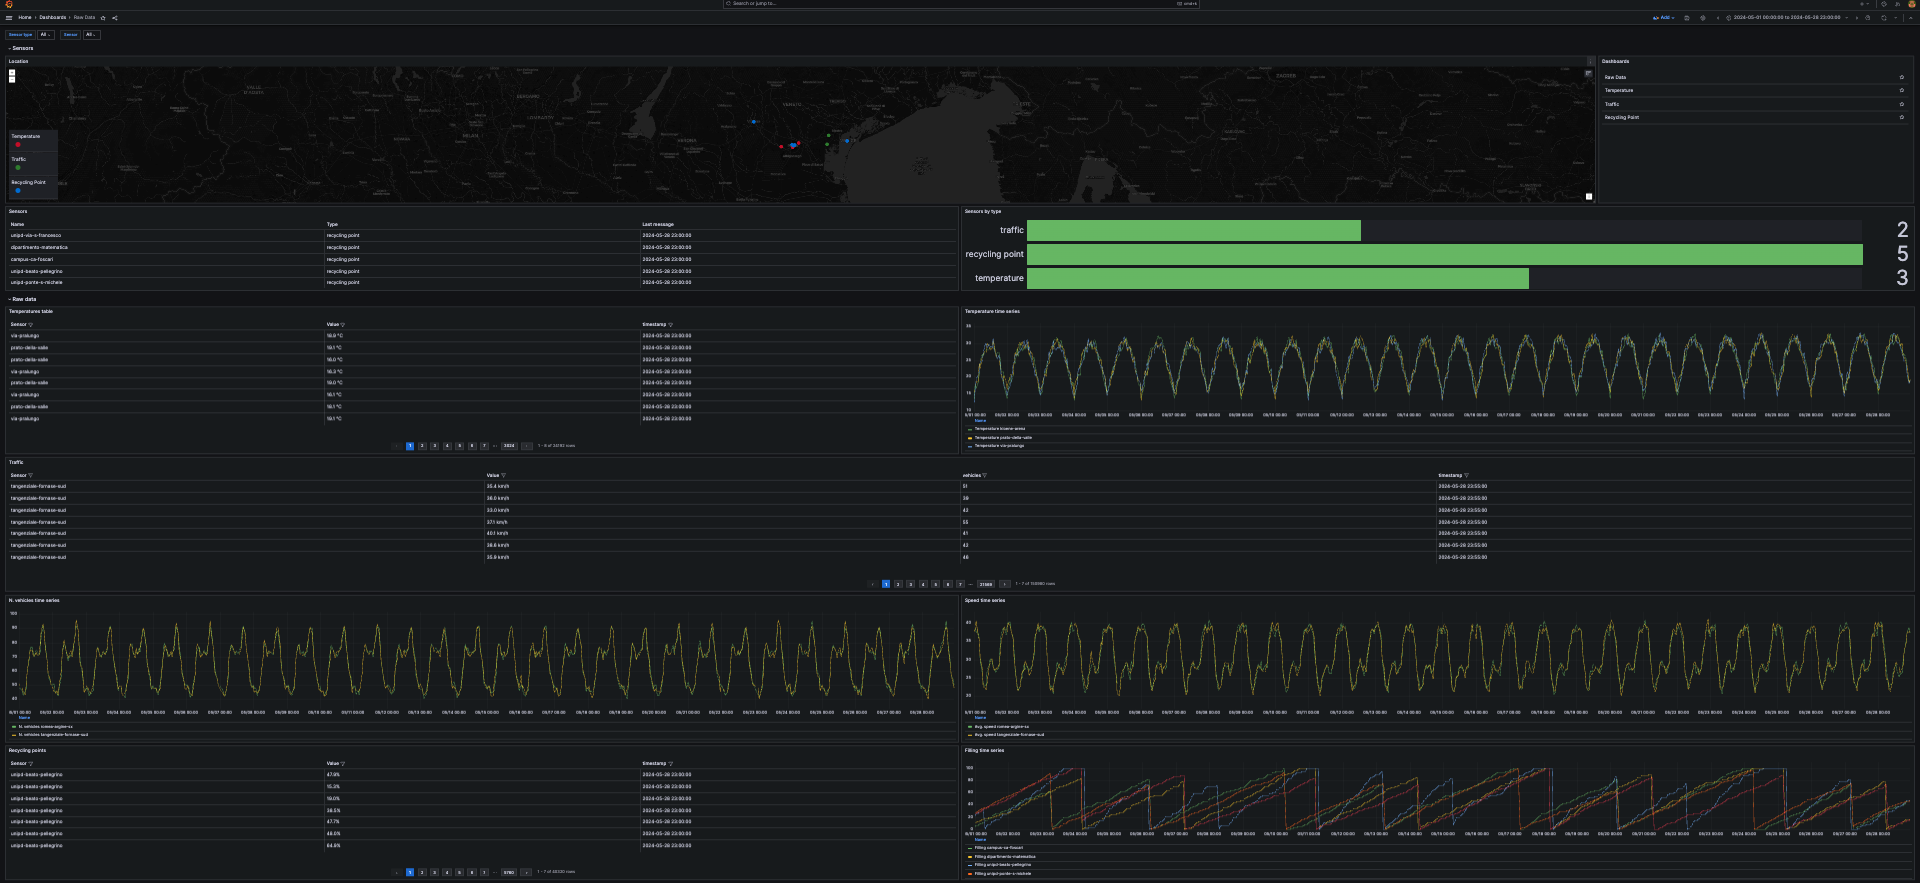
\includegraphics[width=\textwidth]{manuale/general_dashboard.png}
    \captionof{figure}{Dashboard generale}
\end{center}

\newpage
\subsubsection{Isole ecologiche}
Tale dashboard offre una visualizzazione dettagliata delle informazioni sui sensori situati in alcune aree specifiche. Comprende grafici interattivi per monitorare l'andamento delle misurazioni nel tempo e statistiche riassuntive per una panoramica immediata. La sezione \textit{Isole ecologiche}, organizzata dall'alto verso il basso e da sinistra verso destra, è composta da:
\begin{itemize}
    \item filtro per visualizzare i sensori di preferenza;
    \item mappa dei sensori;
    \item grafico a linee con l'andamento del riempimento nel tempo;
    \item percentuale di riempimento attuale;
    \item tempo totale di riempimento;
    \item efficienza delle isole ecologiche;
    \item distribuzione percentuale dei valori di riempimento del sensore in tre intervalli.
\end{itemize}
\begin{center}
    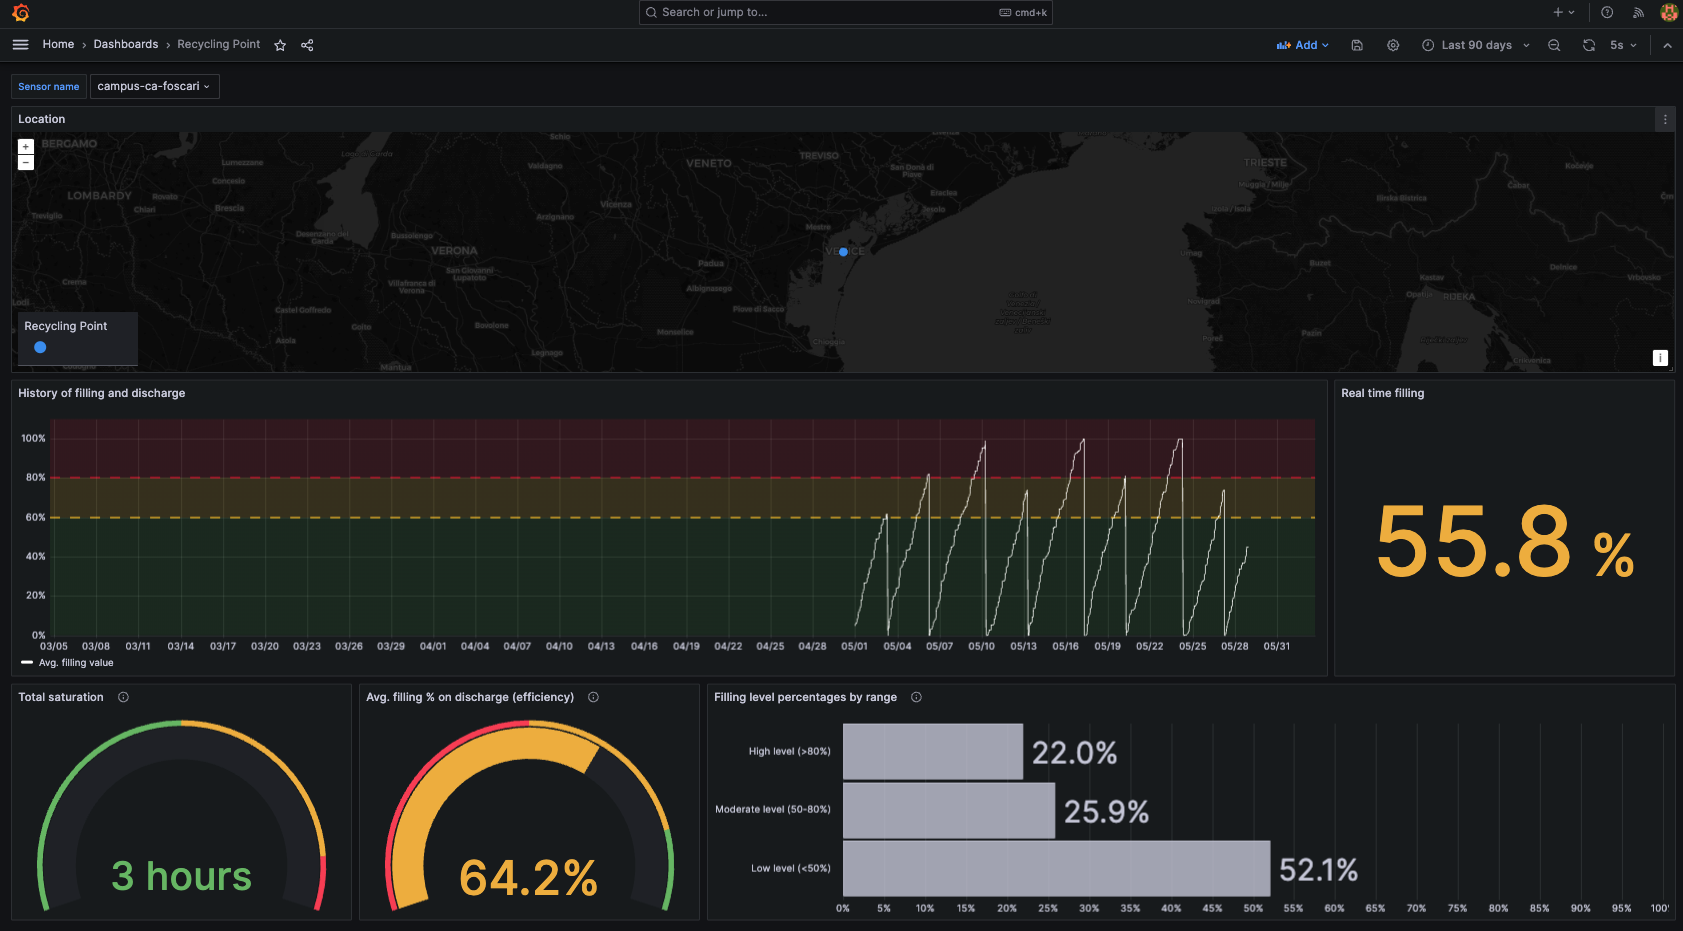
\includegraphics[width=\textwidth]{manuale/eco_ice.png}
    \captionof{figure}{Dashboard Isole ecologiche}
\end{center}

\subsubsection{Temperatura}
La dashboard per la temperatura fornisce una visione dettagliata delle rilevazioni effettuate dai sensori in varie zone. Comprende grafici interattivi per tracciare l'andamento delle misurazioni nel tempo e statistiche riassuntive per un'immediata comprensione. La sezione \textit{Temperatura}, organizzata dall'alto verso il basso e da sinistra verso destra, è composta da:
\begin{itemize}
    \item filtro per visualizzare i sensori di preferenza;
    \item mappa dei sensori;
    \item grafico a linee con l'andamento della temperatura nel tempo;
    \item temperatura attuale;
    \item temperatura media settimanale;
    \item temperatura media giornaliera;
    \item temperatura minima, media e massima.
\end{itemize}
\begin{center}
    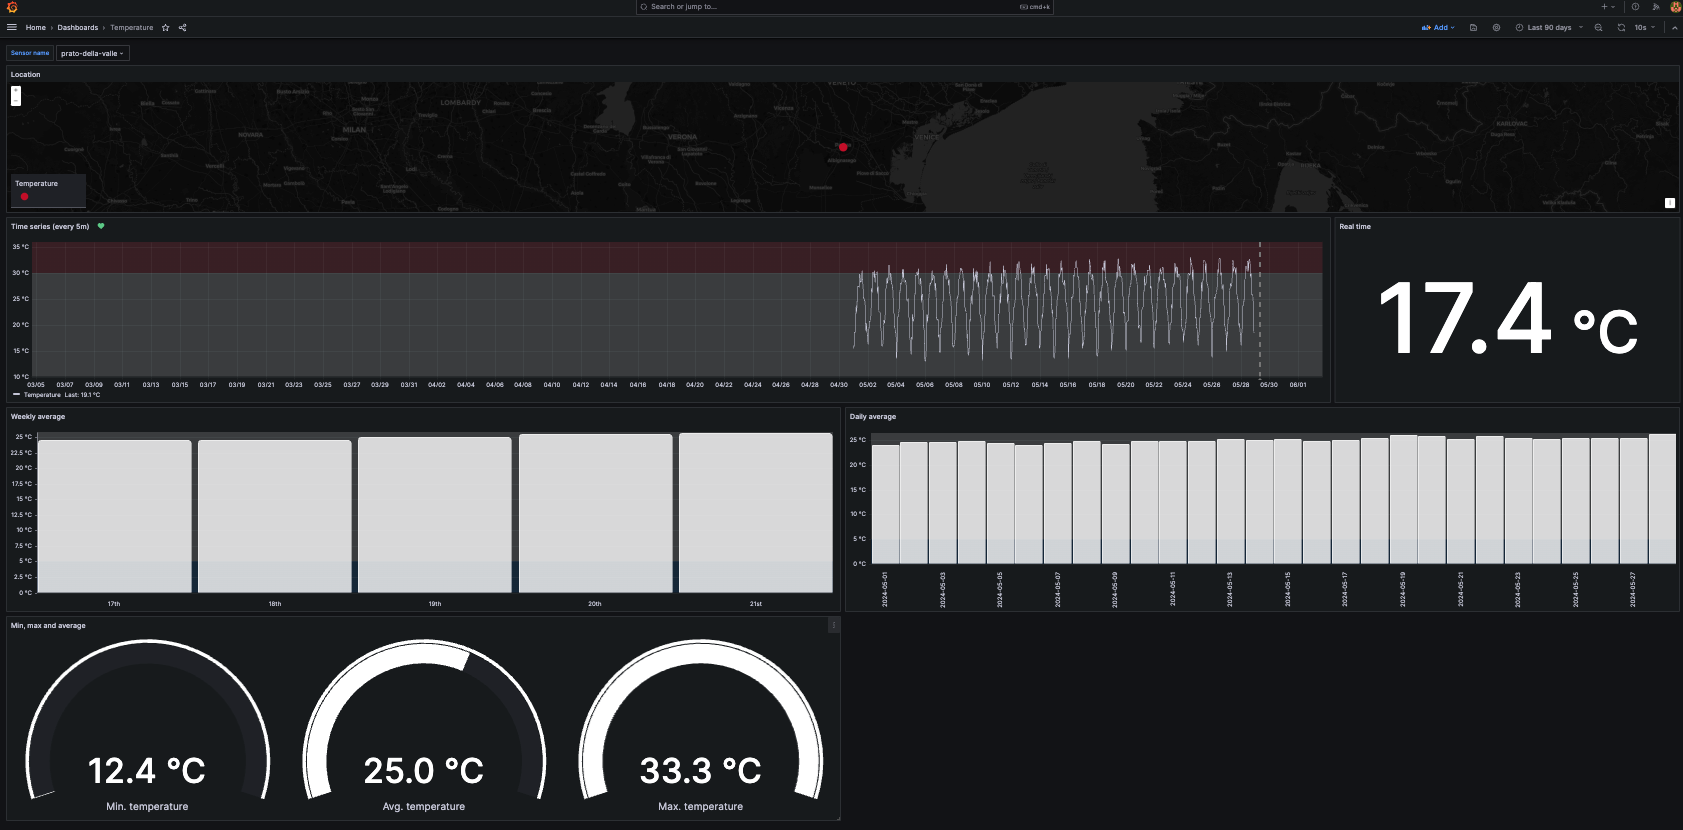
\includegraphics[width=\textwidth]{manuale/temperature.png}
    \captionof{figure}{Dashboard Temperatura}
\end{center}

\newpage
\subsubsection{Traffico}
La dashboard per il traffico fornisce una visualizzazione approfondita dei dati raccolti dai sensori situati in diverse zone. Include grafici interattivi per monitorare l'andamento delle misurazioni nel tempo e statistiche riassuntive per una comprensione immediata. La sezione \textit{Traffico}, disposta dall'alto verso il basso e da sinistra verso destra, è composta da:
\begin{itemize}
    \item filtro per visualizzare i sensori di preferenza;
    \item mappa dei sensori;
    \item numero di veicoli e velocità media in tempo reale;
    \item grafico a barre con il numero di veicoli per ora;
    \item grafico a linee con l'andamento del traffico nel tempo;
    \item grafico a linee con la velocità del traffico nel tempo.
\end{itemize}
\begin{center}
    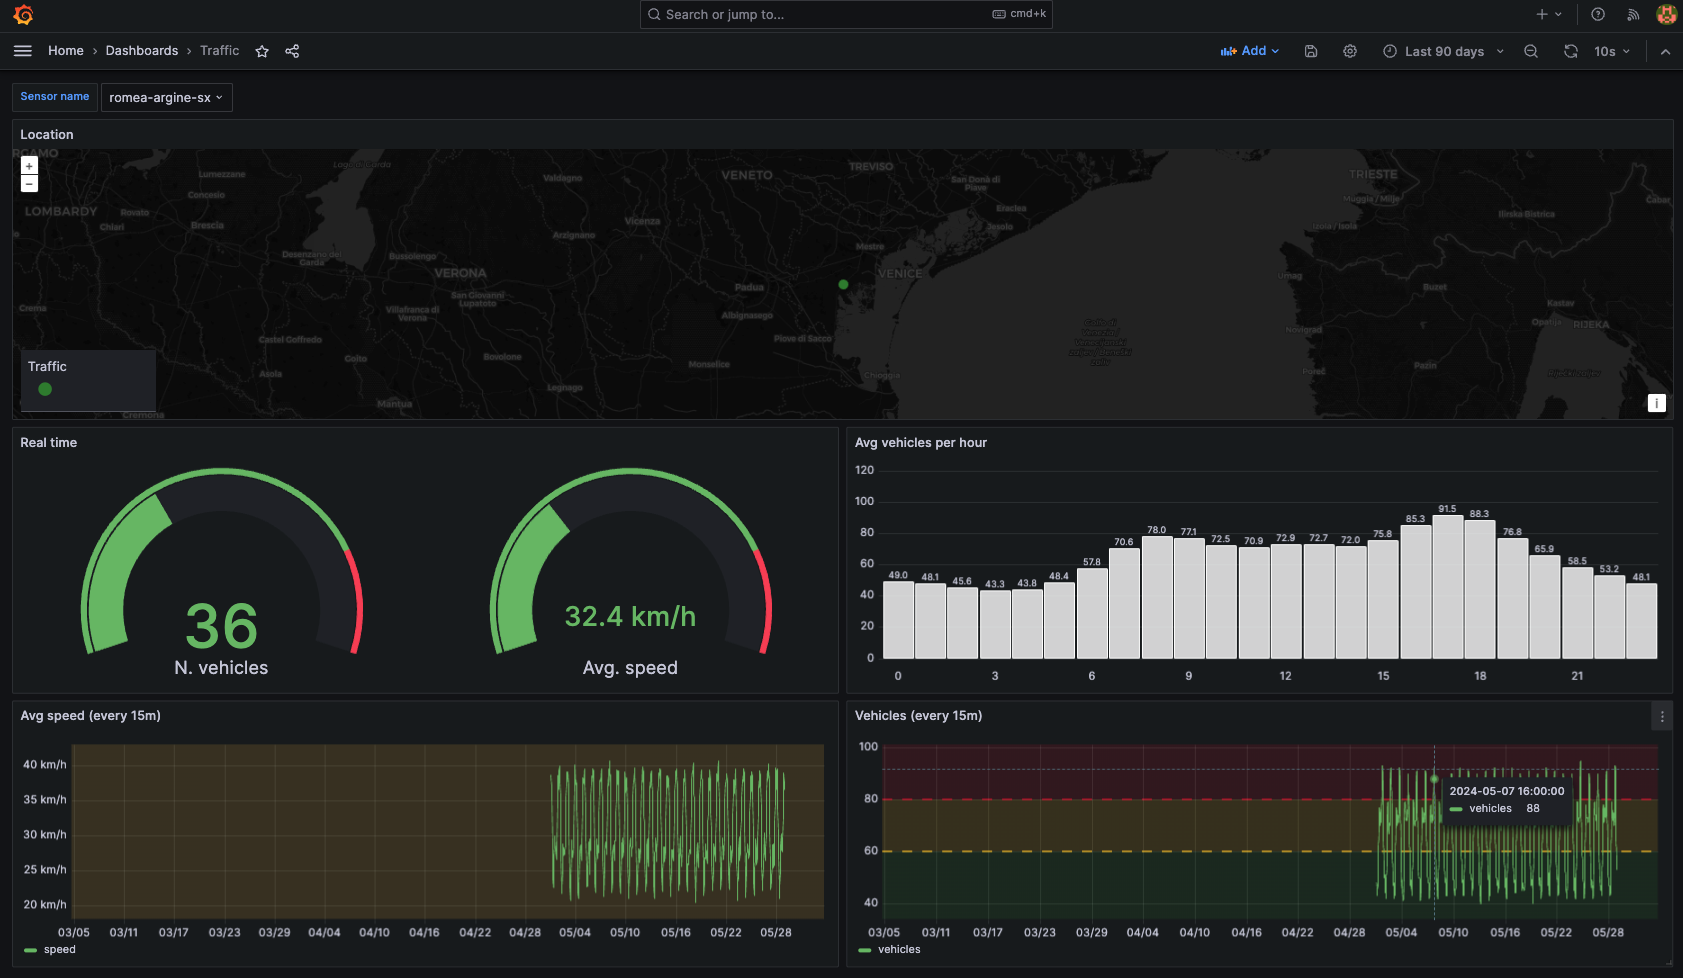
\includegraphics[width=\textwidth]{manuale/traffic.png}
    \captionof{figure}{Dashboard Traffico}
\end{center}


% \subsubsection{Minimizzare e massimizzare i gruppi di pannelli} %Non so se l'abbiamo
% \subsection{Dashboard dettagliate}
% \subsubsection{Accesso alle dashboard dettagliate}
% \subsubsection{Zoom in dashboard}

%--------------------------------------------------------------------%
%TODO da mettere in caso ci facciano inserire il login
% \subsection{Profilo utente}
% \subsubsection{Profile}
% \subsubsection{Notification history}
% \subsubsection{Change password}
%--------------------------------------------------------------------%

\subsection{Alert}
Sono strumenti fondamentali per monitorare le metriche e ricevere notifiche immediate in caso di anomalie o superamento di soglie predefinite. Configurati attraverso regole personalizzabili, gli alert consentono agli utenti di definire condizioni specifiche che, se soddisfatte dai dati monitorati, attivano automaticamente un avviso.
\subsubsection{Visualizzazione}
Gli alert vengono visualizzati nella sezione \textit{Alerting}, dove sono presenti menù espandibili che mostrano il nome dell'alert e lo stato dei vari sensori. Inoltre, nella visualizzazione del grafico \textit{Time Series}, viene mostrata una linea tratteggiata nel momento in cui viene effettuato il check degli allarmi. Questa linea assume un colore diverso a seconda che l'allarme sia stato attivato o meno, fornendo un'indicazione visiva immediata dello stato degli allarmi nel contesto temporale.

\begin{center}
    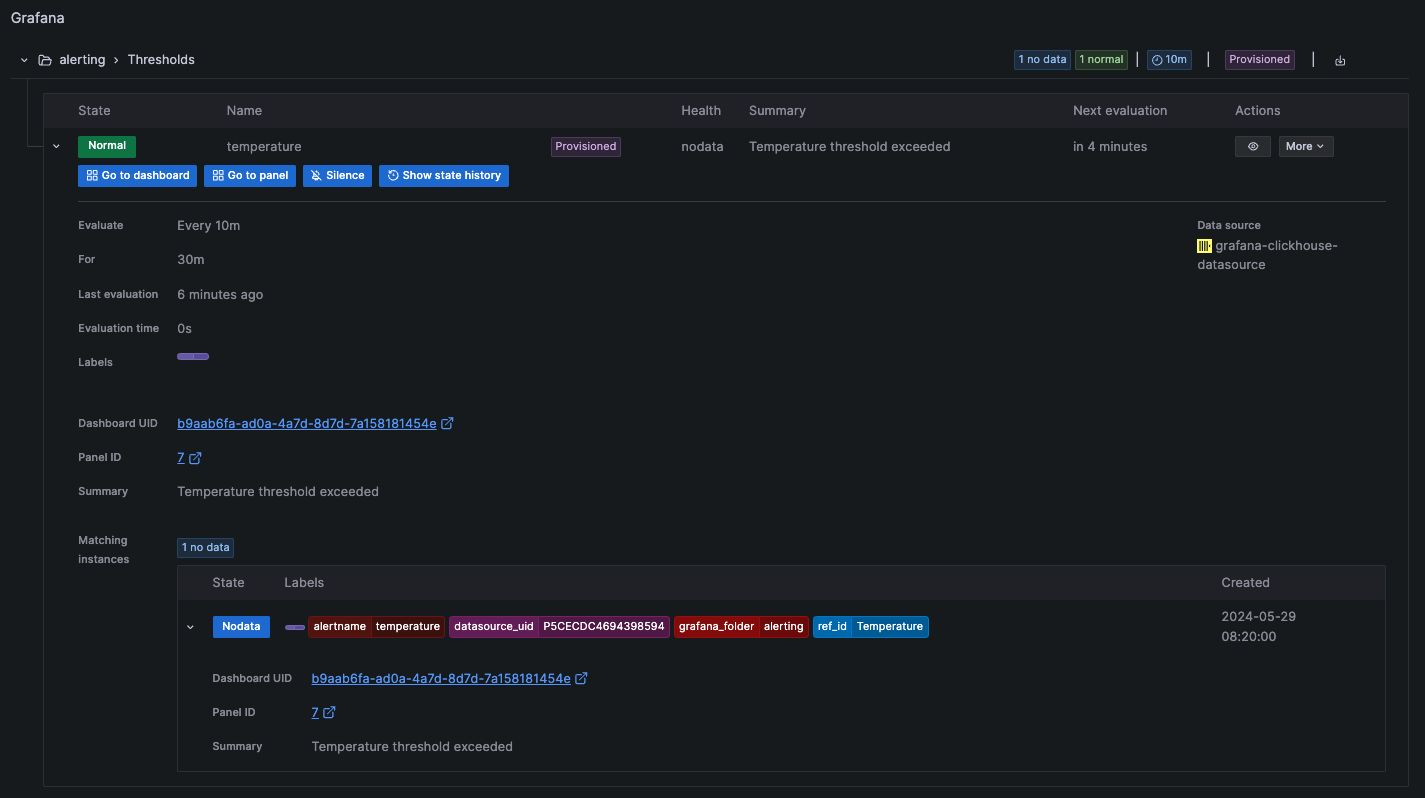
\includegraphics[width=0.6\textwidth]{manuale/alert_grafana.png}
    \captionof{figure}{Alert su Grafana}
\end{center} 

\subsubsection{Notifiche}
La funzionalità di notifica per gli alert è stata integrata per garantire agli utenti di ricevere avvisi tempestivi tramite la piattaforma di loro scelta, come email, Discord e altri canali. Questo sistema avvisa immediatamente in caso di superamento di soglie critiche o anomalie nei dati monitorati, consentendo agli utenti di reagire prontamente a situazioni importanti e garantire la continuità delle operazioni senza interruzioni.
\begin{center}
    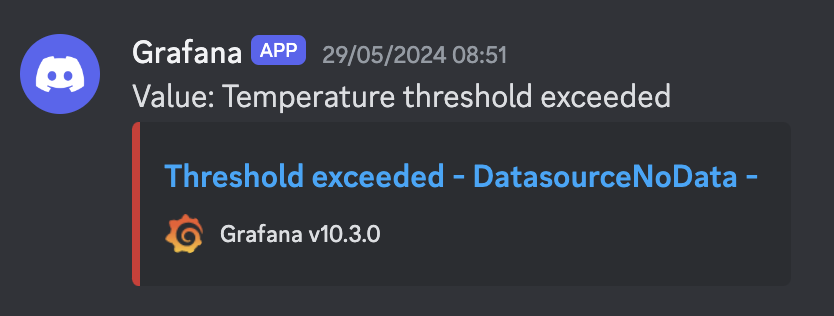
\includegraphics[width=0.6\textwidth]{manuale/notification.png}
    \captionof{figure}{Notifiche Discord}
\end{center} 

\newpage
\section{Supporto}
Per assistenza tecnica o domande relative all’utilizzo dell’applicazione, si prega di contattare il nostro team di supporto all'indirizzo email: 
\begin{center}
    \href{mailto:7last.swe@gmail.com}{7last.swe@gmail.com}
\end{center} 
Per garantire un servizio efficiente e tempestivo, vi invitiamo a includere nel messaggio il maggior numero possibile di dettagli pertinenti. Sarà nostra premura rispondere nel minor tempo possibile.